\chapter{随机变量序列的收敛性}
\begin{introduction}
  \item Intro to Prob\quad5.3 \quad 5.5  
  \item Prob $\&$ Stat\quad4.1
\end{introduction}
\section{引导问题:数列的收敛性 vs 随机变量序列的收敛性}
在高等数学中,我们学习过数列的收敛性。
\begin{definition}{数列的收敛性}
设一个数列$\{a_1,a_2,\cdots,a_n,\cdots\}$。如果对于任意$\varepsilon > 0$,存在一个正整数$n_0$,当$n\geq n_0$时,有
$$
|a_n - a| < \epsilon
$$
则称数列$\{a_n\}$是收敛的,其极限为$a$,记为$\lim_{n\rightarrow \infty } a_n = a$。
\end{definition}
于是,一个很自然的问题:现有一列随机变量$X_1,X_2,\cdots,X_n,\cdots$,其极限是否存在?如何定义随机变量序列的收敛性?
\section{依概率收敛}
我们举一个例子,可以直观感受一下随机变量序列是可以收敛的。
\begin{example}
在抛一枚均匀硬币(正面反面出现的概率相等)的场景下,令随机变量$X_i$表示$i$枚硬币正面朝上的频率。考虑一次实验的数据,如表\ref{tab:Lect11_cointossing10_result}。
\begin{table}[ht]
\centering
\caption{10次抛硬币的结果}\label{tab:Lect11_cointossing10_result}
\begin{tabular}{c cccccc ccccc}
\hline
    第$i$次抛硬币 & 1 & 2 & 3 & 4 & 5 & 6 & 7 & 8 & 9 & 10  \\
\hline
    结果 & 反面 & 反面 & 正面 & 正面 & 反面 & 正面 & 正面 & 正面 & 反面 & 反面\\ 
 \hline
\end{tabular}
\end{table}

于是,根据抛硬不的结果,随机变量序列$\{X_i\}$的取值为$x_i$,见表\ref{tab:Lect11_cointossing10_frequency}
\begin{table}[ht]
\centering
\caption{随机变量序列的取值情况}\label{tab:Lect11_cointossing10_frequency}
\begin{tabular}{c cccccc ccccc}
\hline
    $x_i$ & 1 & 2 & 3 & 4 & 5 & 6 & 7 & 8 & 9 & 10  \\
\hline
    取值 & $0$ & $0$ & $0.33$ & $0.50$ & $0.40$ & $0.50$ & $0.57$ & $0.63$ & $0.56$ & $0.50$\\ 
 \hline
\end{tabular}
\end{table}

根据表\ref{tab:Lect11_cointossing10_frequency},我们可以将$\{X_i\}$绘制在一张图中,如图\ref{fig:Lect11_cointossing10_frequency}。

\begin{figure}[h]
    \centering
    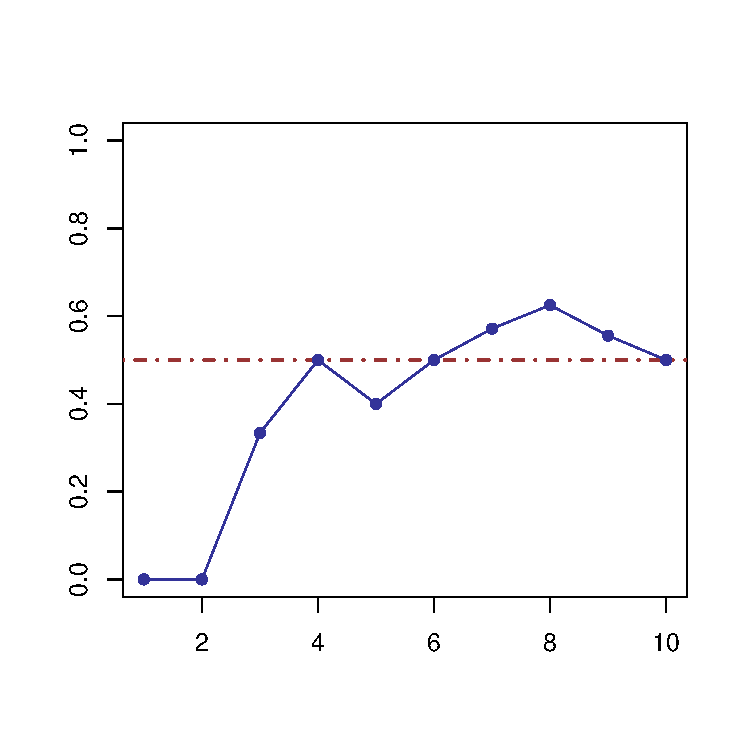
\includegraphics[scale=0.75]{image/Lect11_Coin_Toss.pdf}
    \caption{抛10枚硬币的结果}
    \label{fig:Lect11_cointossing10_frequency}
\end{figure}
\end{example}

\newpage
类似地,我们分别抛30、60、90以及120次硬币后的结果,如图\ref{fig:Lect11_cointossing2}所示。

\begin{figure}[h]
    \centering
    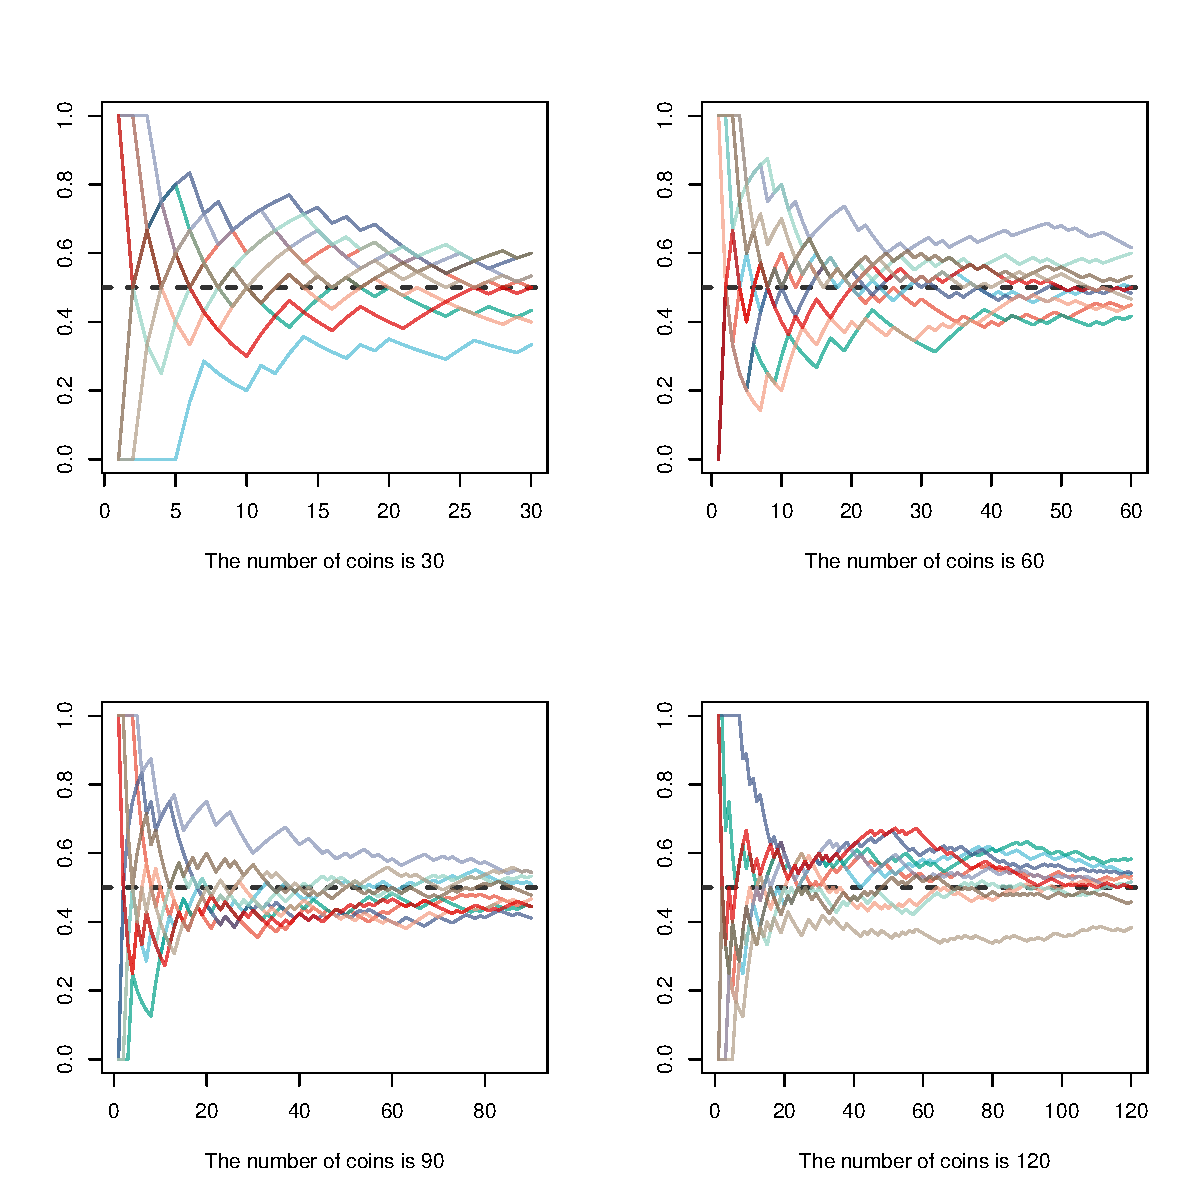
\includegraphics[scale=0.8]{image/Lect11_coin_tossing2.pdf}
    \caption{多次抛硬币的结果}
    \label{fig:Lect11_cointossing2}
\end{figure}

请思考一下以下两个问题:
\begin{problem}
    \begin{enumerate}
        \item 从你运行的实验中,你发现了什么相似点?
        \item 这些相似的结果是否普遍存在的?
    \end{enumerate}
\end{problem}


\begin{conclusion}
    \begin{enumerate}
    \item 概率是频率的稳定值;
    \item 频率$X_n$与概率$p$的绝对偏差$\left|x_{n}-p\right|$将随$n$增大而呈现主键减小的趋势;
    \item 由于随机性,绝对偏差$\left|x_{n}-p\right|$时大时小,虽然无法排除大偏差发生的可能性,但岁$n$不断增大,大偏差发生的可能性会越来越小。
\end{enumerate}
\end{conclusion}


由此,我们定义随机变量序列的一种收敛性。
\begin{definition}
设$\{X_n\}$为一随机变量序列,而$X$为一随机变量。如果对任意的$\varepsilon>0$,有  
$$
\lim _{n \rightarrow \infty} P\left(\left|X_{n}-X\right| \geqslant \varepsilon\right)=0$$

则称序列$\{X_n\}$\textbf{依概率收敛}于$X$,记作$X_{n} \stackrel{P}{\longrightarrow} X$。
\end{definition}
\begin{remark}
\begin{enumerate}
    \item 在定义中$P\left(\left|X_{n}-X\right| \geqslant \varepsilon\right) \rightarrow 0 $,等价于$P\left(\left|X_{n}-X\right|<\varepsilon\right) \rightarrow 1$;
    \item 特别地,$P(X=c)=1$ 时, 则$X_{n}\stackrel{P}{\longrightarrow} c$。
\end{enumerate}    
\end{remark}


\newpage
\begin{property}{(依概率收敛的四则运算)}

设$\{X_n\}, \{Y_n\}$是两个随机变量序列,$a,b$是两个常数。如果
$$X_{n} \stackrel{P}{\longrightarrow} a, \quad Y_{n} \stackrel{P}{\longrightarrow} b,$$
则有
\begin{enumerate}
    \item $X_{n} \pm Y_{n} \stackrel{P}{\rightarrow} a \pm b $;
    \item $X_{n} \times Y_{n} \stackrel{P}{\rightarrow} a \times b $;
    \item $ X_{n} / Y_{n} \stackrel{P}{\rightarrow} a / b, b \neq 0 $。
\end{enumerate}
\end{property}

\begin{example}
设随机变量$X_n$服从柯西分布,其密度函数为
$$p_{n}(x)=\frac{n}{\pi\left(1+n^{2} x^{2}\right)} \quad-\infty<x<\infty.$$
试证$X_{n} \stackrel{P}{\rightarrow} 0$。
\end{example}
\begin{proof}
我们考虑事件$\{|X_n - 0|\geq  \varepsilon\}$发生的概率,即
\begin{eqnarray*}
P\left(\left|X_{n}-0\right| \geq \varepsilon\right) &=&P\left(\left|X_{n}\right| \geqslant \varepsilon\right) \\
&=&\int_{-\infty}^{-\varepsilon} p_{n}(x) d x+\int_{\varepsilon}^{+\infty} p_{n}(x) d x \\
&=&\int_{-\infty}^{-\varepsilon} \frac{n}{\pi\left(1+n^{2} x^{2}\right)} d x+\int_{\varepsilon}^{+\infty} \frac{n}{\pi\left(1+n^{2} x^{2}\right)} d x \\
&=&\frac{2}{\pi} \int_{\varepsilon}^{+\infty} \frac{1}{\pi\left(1+n^{2} x^{2}\right)} d(n x) \\
&\overset{{n x=\tan u}}{=} & \frac{2}{\pi} 
\int_{\operatorname{arctan}(n \varepsilon)}^{\frac{\pi}{2}} \frac{1}{1+\tan ^{2} u} \cdot d \operatorname{tan}u\\
&=&\frac{2}{\pi}\left(\left.u\right|_{\arctan (n \varepsilon)} ^{\frac{\pi}{2}}\right) \\
&=&\frac{2}{\pi}\left(\frac{\pi}{2}-\arctan (n \varepsilon)\right) \\
&=& 1-\frac{2}{\pi} \cdot \arctan (n \varepsilon) \rightarrow 0
\end{eqnarray*}
\end{proof}


\begin{problem}
    比较一下,数列的收敛性与随机变量的收敛性。
    \vspace{5cm}
\end{problem}

\begin{problem}
    如果$X_{n} \stackrel{P}{\rightarrow} a $,那么 $E\left(X_{n}\right) \rightarrow a$成立吗?
\end{problem}

接下来我们看下面一个例子。
\begin{example}
考虑一个随机变量,其分布列为
$$P\left(X_{n}=x\right)=\left\{\begin{aligned}
&1-\frac{1}{n}, & x=0 \\
&\frac{1}{n}, & x=n^{2} \\
&0, & \text{其他}.
\end{aligned}\right.$$
\end{example}
\begin{solution}
由题可知,$$P\left(\left|X_{n}\right|>\varepsilon\right)=P\left(X_{n}=n^{2}\right)=\frac{1}{n} \rightarrow 0.$$
因此,$X_{n} \stackrel{P}{\rightarrow} 0$。我们来计算一下$X_n$的数学期望,即
$$E\left(X_{n}\right)=0 \cdot\left(1-\frac{1}{n}\right)+n^{2} \cdot \frac{1}{n}=n \rightarrow \infty. $$
因此,$E\left(X_{n}\right) \rightarrow 0$。
\end{solution}

\section{按分布收敛}
在学习泊松分布时,泊松分布是二项分布的一种近似,见定理\ref{thm:relation_between_poison_and_binomial}。若设$X_n \sim b(n,p_n)$,其分布函数为$F_n(x)$,且$X \sim P(\lambda)$,$p=\lim_{n\rightarrow} np_n$,其分布函数为$F(x)$。
   对于分布函数序列$\{F_n(x)\}$,根据泊松定理可知,当$n$充分大时,其收敛到一个极限分布函数$F(x)$。

   \begin{note}
        \vspace{3cm}
   \end{note}
\begin{problem}
   如何定义分布函数序列${F_n(x)}$的收敛性?
\end{problem}
一个很自然的想法是——对于任意的$x\in R$,当$n\rightarrow +\infty$时,有
$$
F_n(x) \rightarrow F(x). 
$$
这也就是“点点收敛”,但是这个要求过于严格了。以下例子正好说明了这个问题。

\begin{example}
我们考虑以下随机变量序列$\{X_n\}$的分布列,即
$$P\left(X_{n}=\frac{1}{n}\right)=1 \quad n=1.2, \cdots.$$
于是,其分布函数为
$$F_{n}(x)=\left\{\begin{aligned}
&0,& x<\frac{1}{n}, \\
&1,& x \geqslant \frac{1}{n}.
\end{aligned}\right.$$
那么,对于任意的$x$,$F_n(x)$的极限函数为
$$
g(x)=\left\{\begin{aligned}
&0, & x \leq 0, \\
&1, & x>0.
\end{aligned}\right.$$

然而,我们发现$g(x)$并不满足右连续性,所以,$g(x)$不是一个随机变量的分布函数。由此,随机变量序列的分布函数的极限不是一个随机变量的分布函数,这是不合理的。

我们发现,随机变量$X_n$的分布函数$F_n(x)$是在点$x_0=\frac{1}{n}$处有跳跃点。当$n \rightarrow +\infty$时,跳跃点$x_0 \rightarrow 0$。可以证明
$$
F(x)=\left\{\begin{aligned}
&0, & x<0 \\
&1, & x \geqslant 0
\end{aligned}\right. 
$$
是一个随机变量的分布函数。对于任意的$x \in (-\infty,0)\cup (0,+\infty)$,有$\lim_{n\rightarrow +\infty} F_n(x) = F(x)$。但在$x=0$处,
$$\lim _{n \rightarrow \infty} F_{n}(0)=0 \neq 1=F_{n}(0).$$
\end{example}
 \begin{remark}
 在上面的例子中,分布函数的收敛性不成立的点$x=0$恰好是$F(x)$的间断点(或跳跃点)。我们在定义分布函数的收敛性仅需要考虑$F(x)$的连续点。
 \end{remark}

\begin{definition}
设随机变量$X, X_{1}, X_{2}, \cdots, X_{n}, \cdots$的分布函数分别为$F(x),F_1(x),F_2(x),\cdots,F_n(x),\cdots$。若对$F(x)$的任意连续点$x$,都有
$$\lim _{n \rightarrow \infty} F_{n}(x)=F_{(x)}.$$
则称$F_n(x)$弱收敛与$F(x)$,记作
$$F_{n}(x) \stackrel{\omega}{\longrightarrow} F(x).$$
也称相应的随机变量序列${X_n}$按分布收敛于$X$,
$$X_{n} \stackrel{L}{\longrightarrow} X.$$
\end{definition}
如果$F(x)$是连续函数,那么弱收敛就点点收敛。

\begin{property}
\begin{enumerate}
    \item $X_{n} \stackrel{P}{\rightarrow} X \Rightarrow X_{n} \stackrel{L}{\rightarrow} X$;
    \item 如果$c$是一个常数,那么$X_{n} \stackrel{P}{\rightarrow} c \Leftrightarrow X_{n} \stackrel{L}{\rightarrow} c$。
\end{enumerate}
\end{property}

\section{以概率1收敛(选修)}

\begin{definition}
设$\{X_n\}$是一列随机变量,如果
$$P\left(\lim _{n \rightarrow \infty} X_{n}=X\right)=1$$

则称序列$\{X_n\}$以概率1收敛于$X$,记$X_{n} \stackrel{a \cdot s}{\rightarrow} X$。
\end{definition}
\begin{property}
$X_{n} \stackrel{a \cdot s}{\rightarrow} X \Rightarrow X_{n} \stackrel{P}{\rightarrow} X$,反之不然。
\end{property}

\begin{example}
    考虑一个离散时间的到达过程。我们假定到达的时刻属于正整数集${1,2,\cdots}$。现将这个集合分割成若干个互不相交的集合,$I_{k}=\left\{2^{k}, 2^{k}+1, \cdots, 2^{k+1}-1\right\},k=0,1,\cdots$。注意到集合$I_k$的元素个数为$2^k$,随着$k$的增大而增大。具体来说,
    \begin{eqnarray*}
        I_0 &=& \{1\}\\
        I_{1}&=&\{2,3\}\\
        I_{2}&=&\{4,5,6,7\}\\
        \vdots
    \end{eqnarray*}
    假设在每个区间$I_k$中只有唯一的一个到达时刻,且在区间内每个时刻到达是等可能的。同时假定在各个区间到达时刻是相互独立的。

    记第$k$个区间$I_k$内的到达时刻为$n_k$,则$n_k$是相互独立的随机变量序列,$k=1,2,\cdots$。定义一个新的随机变量序列$\{Y_n\}$,如果时刻$n$到达了,则定义$Y_n = 1$;否则,$Y_n = 0$。如果$n \in I_k$,则$P(Y_n =1) = P(Y_n \neq 0) = \frac{1}{2^k}$。

    接下来,我们来考虑随机变量序列$\{Y_n\}$的收敛性。
    \begin{enumerate}
        \item 因为$I_k$互不相容,对于任意的$n$,存在唯一$k$,使得$n \in I_k$。当$n$越大,则$k$也越大,即
        $$
        \lim_{n\rightarrow +\infty} P(Y_n > \varepsilon) = \lim_{n\rightarrow +\infty} \frac{1}{2^k} = 0.
        $$
        因此,$Y_{n} \stackrel{P}{\longrightarrow} 0 $。
        \item 然而,每个区间$I_k$都有到达时刻,所以,取值为$1$的$Y_n$的个数是无穷多次,即对于任意$N$,存在$n > N$,使得
        $$
        P(Y_n = 1) = 1
        $$
        因此,$P(\lim_{n \rightarrow +\infty} Y_n = 0) \neq 1$,即$Y_n$不以概率$1$收敛到$0$。
    \end{enumerate}
\end{example}
\section{习题}
\begin{enumerate}
    \item 设$D(x)$为退化分布:
$$
D(x) = \left\{ 
	 \begin{matrix}
	 0, &  x < 0,\\
	 1, &  x\geq0.
	 \end{matrix} 
	 \right.
$$
试问下列分布函数列的极限函数是否仍是分布函数?(其中$n = 1,2,\cdots.$)
\begin{enumerate}
    \item $\{D(x + n)\}$;
\item $\{D(x + 1/n)\}$;
\item $\{D(x-1/n)\}.$
\end{enumerate}


\item 设$X_1,X_2,\cdots$是均匀分布于(-1, 1)区间的独立随机变量。证明序列$Y_1,Y_2,\cdots$在概率上收敛到某个极限,并确定以下每种情况下的极限:
\begin{enumerate}
    \item $Y_n = X_n/n$;
\item $Y_n =(X_n)^n$;
\item $Y_n = X_1\cdot X_2\cdots X_n$;
\item $Y_n = \max\{X_1,\cdots,X_n\}$.
\end{enumerate}

\end{enumerate}